\documentclass[12pt]{article}
\usepackage[utf8]{inputenc}
\usepackage{amsmath, amssymb}
\usepackage{xcolor}
\usepackage{geometry}
\usepackage{hyperref}
\usepackage{fancyhdr}
\usepackage{enumitem}
\usepackage{minted} % Code highlighting
\usepackage{booktabs} % Clean tables
\usepackage{tikz}
\usetikzlibrary{shapes, arrows, positioning, automata, arrows.meta, calc}

\geometry{margin=1in}
\hypersetup{colorlinks=true, linkcolor=blue, urlcolor=cyan}

\pagestyle{fancy}
\fancyhf{}
\fancyhead[L]{\textbf{\TOPICTITLE}}
\fancyhead[R]{\thepage}

% -------------------------------
% Topic Metadata
% -------------------------------
\newcommand{\TOPICTITLE}{TCP Congestion Control}
\title{\TOPICTITLE\\\large Study-Ready Notes}
\author{Compiled by Andrew Photinakis}
\date{\today}

\setlength{\headheight}{15pt}

\begin{document}
\maketitle
\tableofcontents
\newpage

% This LaTeX file should be saved at: computer_networks/transport_layer/tcp_congestion_control.tex

\section{TCP AIMD (Additive Increase Multiplicative Decrease)}

\subsection{Basic Approach}
\begin{itemize}
    \item \textbf{Approach}: Senders increase sending rate until packet loss (congestion) occurs, then decrease on loss event
    \item \textbf{Additive Increase}: Increase sending rate by 1 MSS every RTT until loss detected
    \item \textbf{Multiplicative Decrease}: Cut sending rate in half at each loss event
    \item Creates characteristic \textbf{sawtooth pattern} - probing for available bandwidth
\end{itemize}

\subsection{Multiplicative Decrease Details}
\begin{itemize}
    \item \textbf{TCP Reno}: Cut rate in half on loss detected by triple duplicate ACK
    \item \textbf{TCP Tahoe}: Cut rate to 1 MSS when loss detected by timeout
\end{itemize}

\subsection{Why AIMD?}
\begin{itemize}
    \item Distributed, asynchronous algorithm proven to:
    \begin{itemize}
        \item Optimize congested flow rates network-wide
        \item Have desirable stability properties
        \item Converge to fair allocation among competing flows
    \end{itemize}
\end{itemize}

\begin{figure}[h]
    \centering
    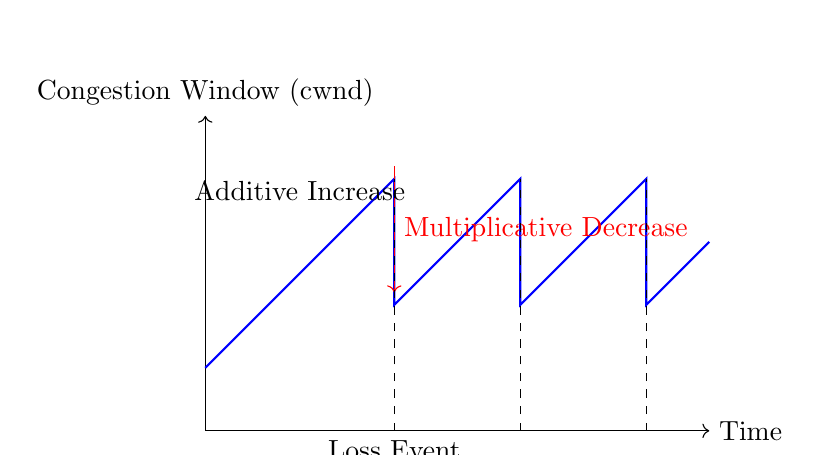
\begin{tikzpicture}[scale=0.8]
        \draw[->] (0,0) -- (8,0) node[right] {Time};
        \draw[->] (0,0) -- (0,5) node[above] {Congestion Window (cwnd)};
        
        % AIMD sawtooth pattern
        \draw[thick, blue] (0,1) -- (1,2) -- (2,3) -- (3,4) -- (3,2) -- (4,3) -- (5,4) -- (5,2) -- (6,3) -- (7,4) -- (7,2) -- (8,3);
        
        % Labels
        \node[above] at (1.5,3.5) {Additive Increase};
        \draw[->, red] (3,4.2) -- (3,2.2) node[midway,right] {Multiplicative Decrease};
        \node[below] at (3,0) {Loss Event};
        
        \foreach \x/\y in {3/4, 5/4, 7/4} {
            \draw[dashed] (\x,0) -- (\x,4);
        }
        
    \end{tikzpicture}
    \caption{AIMD sawtooth behavior: probing for available bandwidth}
    \label{fig:aimd_sawtooth}
\end{figure}

\textcolor{blue}{[Summary: AIMD is TCP's core congestion control mechanism where senders gradually increase rates until congestion occurs, then dramatically reduce rates, creating a stable sawtooth pattern that fairly shares bandwidth.]}

\section{TCP Congestion Control Details}

\subsection{Congestion Window (cwnd)}
\begin{itemize}
    \item Dynamic limit on amount of unacknowledged data
    \item TCP sending rate approximately: \(\text{Rate} \approx \frac{\text{cwnd}}{\text{RTT}}\) bytes/sec
    \item Sender constraint: \(\text{LastByteSent} - \text{LastByteAcked} \leq \text{cwnd}\)
\end{itemize}

\begin{figure}[h]
    \centering
    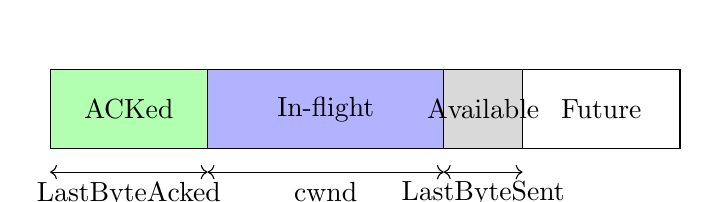
\begin{tikzpicture}
        \draw (0,0) rectangle (8,1);
        \draw[fill=green!30] (0,0) rectangle (2,1);
        \draw[fill=blue!30] (2,0) rectangle (5,1);
        \draw[fill=gray!30] (5,0) rectangle (6,1);
        \draw (6,0) -- (6,1);
        
        \node at (1,0.5) {ACKed};
        \node at (3.5,0.5) {In-flight};
        \node at (5.5,0.5) {Available};
        \node at (7,0.5) {Future};
        
        \draw[<->] (0,-0.3) -- node[below] {LastByteAcked} (2,-0.3);
        \draw[<->] (2,-0.3) -- node[below] {cwnd} (5,-0.3);
        \draw[<->] (5,-0.3) -- node[below] {LastByteSent} (6,-0.3);
        
    \end{tikzpicture}
    \caption{TCP sender sequence number space with congestion window}
    \label{fig:cwnd_window}
\end{figure}

\section{TCP Slow Start}

\subsection{Initial Phase}
\begin{itemize}
    \item When connection begins, increase rate exponentially until first loss
    \item Initial \(\text{cwnd} = 1\) MSS
    \item Double cwnd every RTT
    \item Achieved by incrementing cwnd for every ACK received
\end{itemize}

\subsection{Exponential Growth}
\[
\text{cwnd}_{\text{after RTT}} = \text{cwnd} \times 2
\]
\[
\text{cwnd}_{\text{after n RTTs}} = 2^n \times \text{MSS}
\]

\begin{figure}[h]
    \centering
    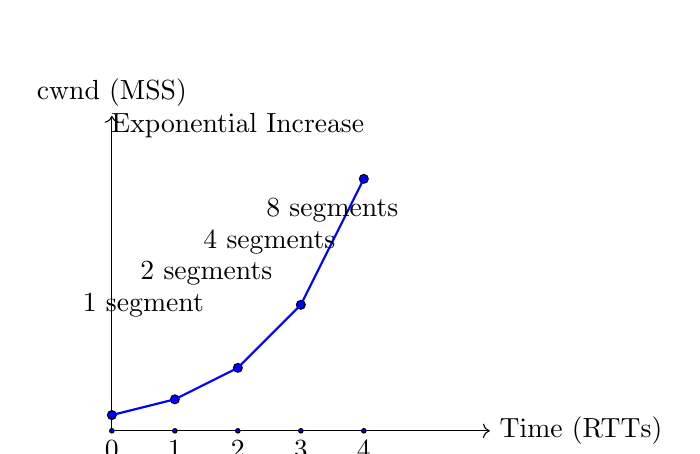
\begin{tikzpicture}[scale=0.8]
        \draw[->] (0,0) -- (6,0) node[right] {Time (RTTs)};
        \draw[->] (0,0) -- (0,5) node[above] {cwnd (MSS)};
        
        % Exponential growth
        \foreach \x/\y in {0/1, 1/2, 2/4, 3/8, 4/16} {
            \draw[fill=blue] (\x,0) circle (1pt);
            \node[below] at (\x,0) {\x};
            \draw[fill=blue] (\x,\y/4) circle (2pt);
        }
        
        \draw[thick, blue] (0,0.25) -- (1,0.5) -- (2,1) -- (3,2) -- (4,4);
        
        % Transmission visualization
        \node at (0.5,2) {1 segment};
        \node at (1.5,2.5) {2 segments};
        \node at (2.5,3) {4 segments};
        \node at (3.5,3.5) {8 segments};
        
        \node[above] at (2,4.5) {Exponential Increase};
        
    \end{tikzpicture}
    \caption{TCP slow start: exponential growth of congestion window}
    \label{fig:slow_start}
\end{figure}

\textcolor{orange}{[Mnemonic: "Slow Start Speeds Up" - Despite the name, slow start actually increases the window exponentially fast, not slowly.]}

\section{TCP Congestion Avoidance}

\subsection{Transition from Slow Start}
\begin{itemize}
    \item Switch from exponential to linear increase when cwnd reaches half its pre-loss value
    \item \textbf{ssthresh} (slow start threshold) variable tracks this point
    \item On loss event: \(\text{ssthresh} = \frac{\text{cwnd}}{2}\)
\end{itemize}

\subsection{Congestion Control States}
\begin{itemize}
    \item \textbf{Slow Start}: Exponential increase until ssthresh
    \item \textbf{Congestion Avoidance}: Additive increase (AIMD)
    \item \textbf{Fast Recovery}: Handling duplicate ACKs
\end{itemize}

\section{TCP Congestion Control Finite State Machine}

\begin{figure}[h]
    \centering
    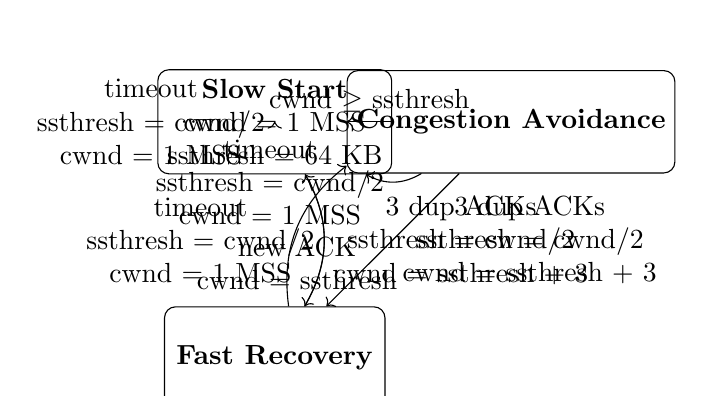
\begin{tikzpicture}[
        node distance=3cm,
        state/.style={
            rectangle,
            draw,
            rounded corners,
            minimum width=2.8cm,
            minimum height=1.3cm,
            align=center
        }
    ]
        % States
        \node[state] (slow_start) {\textbf{Slow Start}\\cwnd = 1 MSS\\ssthresh = 64 KB};
        \node[state, right of=slow_start] (cong_avoid) {\textbf{Congestion Avoidance}};
        \node[state, below of=slow_start] (fast_recovery) {\textbf{Fast Recovery}};
        
        % Transitions
        \draw[->] (slow_start) -- node[above] {cwnd $\geq$ ssthresh} (cong_avoid);
        \draw[->] (slow_start) to[bend right] node[left, align=center] {timeout\\ssthresh = cwnd/2\\cwnd = 1 MSS} (slow_start);
        \draw[->] (slow_start) to[bend left] node[right, align=center] {3 dup ACKs\\ssthresh = cwnd/2\\cwnd = ssthresh + 3} (fast_recovery);
        
        \draw[->] (cong_avoid) to[bend left] node[left, align=center] {timeout\\ssthresh = cwnd/2\\cwnd = 1 MSS} (slow_start);
        \draw[->] (cong_avoid) -- node[right, align=center] {3 dup ACKs\\ssthresh = cwnd/2\\cwnd = ssthresh + 3} (fast_recovery);
        
        \draw[->] (fast_recovery) to[bend left] node[below, align=center] {new ACK\\cwnd = ssthresh} (cong_avoid);
        \draw[->] (fast_recovery) to[bend right] node[left, align=center] {timeout\\ssthresh = cwnd/2\\cwnd = 1 MSS} (slow_start);
        
    \end{tikzpicture}
    \caption{TCP congestion control finite state machine}
    \label{fig:tcp_cc_fsm}
\end{figure}


\section{TCP CUBIC}

\subsection{Motivation for Improvement}
\begin{itemize}
    \item Is there a better way than AIMD to "probe" for usable bandwidth?
    \item Key insight: After cutting rate on loss, initially ramp to \(W_{\text{max}}\) faster, then approach more slowly
    \item \(W_{\text{max}}\): Sending rate at which congestion loss was detected
\end{itemize}

\subsection{CUBIC Algorithm}
\begin{itemize}
    \item \(K\): Point in time when window will reach \(W_{\text{max}}\)
    \item Increase window as cube of distance from current time to \(K\)
    \item Larger increases when further from \(K$, smaller increases when nearer
\end{itemize}

\[
W(t) = C(t - K)^3 + W_{\text{max}}
\]
Where \(C\) is a scaling constant.

\begin{figure}[h]
    \centering
    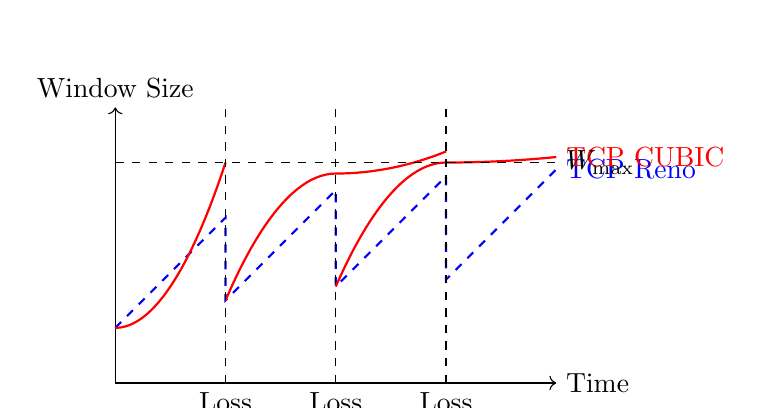
\begin{tikzpicture}[scale=0.7]
        \draw[->] (0,0) -- (8,0) node[right] {Time};
        \draw[->] (0,0) -- (0,5) node[above] {Window Size};
        
        % Classic TCP
        \draw[thick, blue, dashed] (0,1) -- (2,3) -- (2,1.5) -- (4,3.5) -- (4,1.75) -- (6,3.75) -- (6,1.875) -- (8,3.875);
        \node[blue, right] at (8,3.875) {TCP Reno};
        
        % CUBIC
        \draw[thick, red] (0,1) parabola (2,4);
        \draw[thick, red] (2,1.5) parabola bend (4,3.8) (6,4.2);
        \draw[thick, red] (4,1.75) parabola bend (6,4) (8,4.1);
        \node[red, right] at (8,4.1) {TCP CUBIC};
        
        % W_max line
        \draw[dashed] (0,4) -- (8,4) node[right] {$W_{\text{max}}$};
        
        \foreach \x in {2,4,6} {
            \draw[dashed] (\x,0) -- (\x,5);
        }
        
        \node[below] at (2,0) {Loss};
        \node[below] at (4,0) {Loss};
        \node[below] at (6,0) {Loss};
        
    \end{tikzpicture}
    \caption{TCP CUBIC vs classic TCP: CUBIC achieves higher throughput}
    \label{fig:tcp_cubic}
\end{figure}

\subsection{Deployment Status}
\begin{itemize}
    \item Default TCP in Linux
    \item Most popular TCP for popular web servers
    \item Provides better performance on high-bandwidth, high-latency networks
\end{itemize}

\textcolor{blue}{[Summary: TCP CUBIC improves upon AIMD by using a cubic growth function that initially recovers quickly after loss then approaches the previous maximum more cautiously, providing better performance on modern networks.]}

\section{Bottleneck Link Concept}

\subsection{Network Bottlenecks}
\begin{itemize}
    \item TCP increases sending rate until packet loss occurs at some router's output
    \item This congested router is the \textbf{bottleneck link}
    \item Understanding congestion requires focusing on bottleneck links
\end{itemize}

\subsection{Key Insights}
\begin{itemize}
    \item Increasing TCP sending rate beyond bottleneck capacity won't increase end-to-end throughput
    \item Increasing TCP sending rate will increase measured RTT due to queueing
    \item Goal: "Keep the end-end pipe just full, but not fuller"
\end{itemize}

\begin{figure}[h]
    \centering
    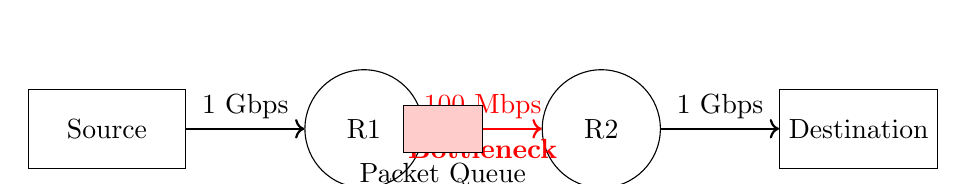
\begin{tikzpicture}[
        node distance=2cm,
        host/.style={rectangle, draw, minimum width=2cm, minimum height=1cm},
        router/.style={circle, draw, minimum size=1.5cm}
    ]
        \node[host] (source) {Source};
        \node[router, right=1.5cm of source] (router1) {R1};
        \node[router, right=1.5cm of router1] (router2) {R2};
        \node[host, right=1.5cm of router2] (dest) {Destination};
        
        % Links with different capacities
        \draw[->, thick] (source) -- node[above] {1 Gbps} (router1);
        \draw[->, thick, red] (router1) -- node[above] {100 Mbps} node[below] {\textbf{Bottleneck}} (router2);
        \draw[->, thick] (router2) -- node[above] {1 Gbps} (dest);
        
        % Queue at bottleneck
        \draw[fill=red!20] ($(router1)+(0.5,-0.3)$) rectangle ($(router1)+(1.5,0.3)$);
        \node at ($(router1)+(1,-0.6)$) {Packet Queue};
        
    \end{tikzpicture}
    \caption{Bottleneck link concept: the slowest link determines maximum throughput}
    \label{fig:bottleneck}
\end{figure}

\section{Delay-Based TCP Congestion Control}

\subsection{Philosophy}
\begin{itemize}
    \item Keep sender-to-receiver pipe "just full enough, but no fuller"
    \item Keep bottleneck link busy transmitting, but avoid high delays/buffering
    \item Congestion control without inducing/forcing loss
\end{itemize}

\subsection{Algorithm Approach}
\begin{itemize}
    \item Measure \(\text{RTT}_{\text{min}}\): Minimum observed RTT (uncongested path)
    \item Calculate uncongested throughput: \(\frac{\text{cwnd}}{\text{RTT}_{\text{min}}}\)
    \item Compare measured throughput with uncongested throughput:
    \begin{itemize}
        \item If "very close": Increase cwnd linearly (path not congested)
        \item If "far below": Decrease cwnd linearly (path congested)
    \end{itemize}
\end{itemize}

\subsection{Deployment Examples}
\begin{itemize}
    \item BBR (Bottleneck Bandwidth and Round-trip propagation time)
    \item Deployed on Google's internal backbone network
    \item Better performance for latency-sensitive applications
\end{itemize}

\section{Explicit Congestion Notification (ECN)}

\subsection{Network-Assisted Approach}
\begin{itemize}
    \item Routers provide direct congestion feedback
    \item Two bits in IP header (ToS field) marked by network router
    \item Congestion indication carried to destination
    \item Destination sets ECE bit on ACK to notify sender
\end{itemize}

\begin{figure}[h]
    \centering
    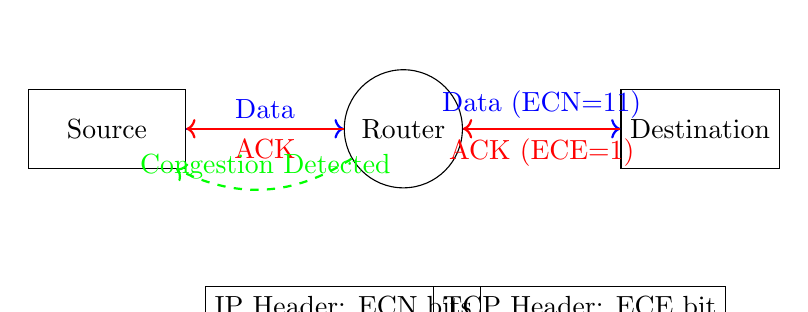
\begin{tikzpicture}[
        node distance=2cm,
        host/.style={rectangle, draw, minimum width=2cm, minimum height=1cm},
        router/.style={circle, draw, minimum size=1.5cm}
    ]
        \node[host] (source) {Source};
        \node[router, right=2cm of source] (router) {Router};
        \node[host, right=2cm of router] (dest) {Destination};
        
        % Data flow with ECN marking
        \draw[->, thick, blue] (source) -- node[above] {Data} (router);
        \draw[->, thick, blue] (router) -- node[above] {Data (ECN=11)} (dest);
        
        % ACK flow with ECE
        \draw[->, thick, red] (dest) -- node[below] {ACK (ECE=1)} (router);
        \draw[->, thick, red] (router) -- node[below] {ACK} (source);
        
        % Congestion feedback
        \draw[->, thick, green, dashed] (router) to[bend left=30] node[above] {Congestion Detected} (source);
        
        % IP and TCP headers
        \node[draw, rectangle, below=0.5cm of router] (ip_header) at (3,-1.5) {IP Header: ECN bits};
        \node[draw, rectangle, below=0.5cm of dest] (tcp_header) at (6,-1.5) {TCP Header: ECE bit};
        
    \end{tikzpicture}
    \caption{Explicit Congestion Notification (ECN) mechanism}
    \label{fig:ecn}
\end{figure}

\section{TCP Fairness}

\subsection{Fairness Goal}
\begin{itemize}
    \item If \(K\) TCP sessions share bottleneck link of bandwidth \(R\), each should have average rate of \(R/K\)
    \item TCP converges to fair allocation under idealized conditions
\end{itemize}

\subsection{Fairness Analysis}
\begin{itemize}
    \item Additive increase gives slope of 1 as throughput increases
    \item Multiplicative decrease reduces throughput proportionally
    \item Result: Competing flows converge to equal shares
\end{itemize}

\subsection{Limitations and Violations}
\begin{itemize}
    \item \textbf{UDP applications}: Multimedia apps don't use TCP congestion control
    \item \textbf{Parallel TCP connections}: Applications can open multiple connections
    \item Example: Link with rate R and 9 existing connections:
    \begin{itemize}
        \item New app with 1 TCP gets rate R/10
        \item New app with 11 TCPs gets rate R/2
    \end{itemize}
    \item No "Internet police" enforcing congestion control use
\end{itemize}

\begin{table}[h]
    \centering
    \begin{tabular}{p{0.3\textwidth}p{0.3\textwidth}p{0.3\textwidth}}
        \toprule
        \textbf{Congestion Control Type} & \textbf{Mechanism} & \textbf{Characteristics} \\
        \midrule
        Classic TCP (Reno) & Loss-based AIMD & Sawtooth pattern, proven fairness \\
        TCP CUBIC & Cubic growth function & Better high-speed performance \\
        Delay-based (BBR) & RTT measurements & Lower latency, no forced loss \\
        ECN-enabled & Network feedback & Early congestion notification \\
        \bottomrule
    \end{tabular}
    \caption{Comparison of TCP congestion control variants}
    \label{tab:tcp_cc_variants}
\end{table}

\section{TCP Throughput Analysis}

\subsection{Average Throughput Formula}
Ignoring slow start and assuming always data to send:
\[
\text{Average TCP throughput} = \frac{3}{4} \cdot \frac{W}{\text{RTT}} \quad \text{bytes/sec}
\]
Where:
\begin{itemize}
    \item \(W\): Window size where loss occurs
    \item Average window size is \(\frac{3}{4}W\)
    \item Average throughput is \(\frac{3}{4}W\) per RTT
\end{itemize}

\subsection{Throughput Example}
For a connection with:
\begin{itemize}
    \item Loss window \(W = 10\) MSS
    \item RTT = 100 ms
    \item MSS = 1460 bytes
\end{itemize}
\[
\text{Average throughput} = \frac{3}{4} \cdot \frac{10 \times 1460}{0.1} = 109,500 \text{ bytes/sec} \approx 876 \text{ kbps}
\]

\textcolor{teal}{[Concept Map: TCP Congestion Control → AIMD (core algorithm) + Slow Start (initial phase) + Congestion Avoidance (steady state) + Enhancements (CUBIC, BBR, ECN) → Goals: Efficiency + Fairness + Stability → Prevents congestion collapse while maximizing network utilization.]}

\section{Study Aids and Exam Preparation}

\subsection{Key Concepts to Master}
\begin{itemize}
    \item Understand AIMD mechanism and why it creates sawtooth pattern
    \item Differentiate between slow start and congestion avoidance
    \item Explain TCP CUBIC improvements over classic TCP
    \item Compare loss-based vs delay-based congestion control
    \item Describe ECN mechanism and benefits
    \item Analyze TCP fairness and its limitations
\end{itemize}

\subsection{Practice Questions}
\begin{enumerate}
    \item \textbf{Explain the AIMD mechanism} and draw the characteristic sawtooth pattern. Why does this pattern emerge, and what are its stability properties?
    
    \item Compare \textbf{TCP slow start} and \textbf{congestion avoidance}. When does the transition occur, and what triggers it?
    
    \item Calculate the \textbf{average TCP throughput} for a connection that experiences loss when cwnd = 16 MSS, with RTT = 50 ms and MSS = 1500 bytes.
    
    \item Describe how \textbf{TCP CUBIC} improves upon classic TCP congestion control. What is the key insight behind its cubic growth function?
    
    \item Explain the \textbf{fairness limitations} of TCP congestion control. How can applications "cheat" the system, and what are the implications?
\end{enumerate}

\textcolor{orange}{[Mnemonic: "AIMD: Add Incrementally, Multiply Down" - Add 1 MSS per RTT when increasing, multiply by 0.5 when decreasing.]}

\section{Summary}

\begin{itemize}
    \item TCP congestion control prevents network collapse while maximizing utilization
    \item AIMD (Additive Increase Multiplicative Decrease) is the core algorithm
    \item Slow start provides exponential initial growth
    \item Congestion avoidance provides linear increase after threshold
    \item TCP CUBIC improves performance on high-speed networks
    \item Delay-based approaches (BBR) avoid forced packet loss
    \item ECN enables network-assisted congestion notification
    \item TCP achieves fairness under idealized conditions
    \item Various enhancements address limitations of classic approaches
    \item Throughput can be modeled mathematically based on loss window and RTT
\end{itemize}

\end{document}